\makeatletter
\newif\ifGm@compatii
\makeatother
\documentclass[12pt,landscape,english]{beamer}
\setbeameroption{show notes}


\usepackage{palatino}
\usepackage[T1]{fontenc}
\usepackage{bbding}
\usepackage{etoolbox, verbatim}

\usepackage{tikz}
\usetikzlibrary{positioning, fit,arrows,chains,shapes.geometric}
\usetikzlibrary{graphs,graphdrawing}
%\usetikzlibrary{decorations.text}
\usetikzlibrary{petri}
\usegdlibrary{force, layered, trees}


\usepackage[backend=bibtex, 
bibstyle=ieee,citestyle=verbose-note,firstinits=true]{biblatex}
\bibliography{../../../Resources/master_bibliography/master.bib}

\renewcommand{\footnotesize}{\scriptsize}

\mode<presentation>

%\usetheme[navmenu]{uwa_eng} 
\usetheme{Berkeley}

\setbeamertemplate{itemize item}{\raisebox{-2px}{\JackStarBold} \hskip -.2em}
\setbeamertemplate{itemize subitem}{\raisebox{-2px}{\FourAsterisk} \hskip -.2em}
\setbeamertemplate{itemize subsubitem}{\raisebox{-2px}{\JackStar} \hskip -.2em}


\usepackage{graphicx}
\graphicspath{{../figs/}}


\makeatletter

\definecolor{myframe}{rgb}{0.2,0.2,0.2}  % charcoal frametitle
\setbeamercolor{frametitle}{fg=myframe}
\definecolor{mystruc}{rgb}{0,0.25,0.45}  % turquoise
\usecolortheme[named=mystruc]{structure} 

\setbeamercolor{title}{fg=black}
\usefonttheme{structuresmallcapsserif}



\begin{document}
	
% Titlepage info

\title[Semantic Vector Representations]{Semantic Vector Representations for Natural Language}
\author[L.~White]{
	Lyndon White \texorpdfstring{\\\medskip{\scriptsize Supervised by:\\ Prof Roberto Togneri\\ Dr Wei Liu\\W/Prof Mohammed Bennamoun\\ }}{}}

\date{} % show no date
%\titlegraphic{\includegraphics[width=2.1cm]{balls}}
{
\usebackgroundtemplate{\includegraphics[width=\paperwidth,height=\paperheight]{uwa_eng_title.png}}
\begin{frame}[plain]
	\titlepage
\end{frame}
}

%%%%%%%%%%%%%%%%%%%%Definitions

\def\x{\tilde{x}}
\def\y{\tilde{y}}
\def\b{\tilde{b}}


%%%%%%%%%%%%%%%%%%%%%%%%%%%%


\section{Introduction}
\begin{frame} {Why Natural Language Understanding?} 
	\vspace{-1cm}
	
	\note{Shown are two lists of information. On one side are examples of informaition in a form easily accessable by software. On the other is information recored digitally in natural language.
		}
\begin{columns}
	\begin{column}{0.5\textwidth}
		\center\resizebox{0.4\textwidth}{!}{\includegraphics{pres/people.png}}
		\begin{itemize}
			\item $10^7$ {\small StackOverflow QAs}
			\item $10^7$ Digitalised Books \note[item]{Google has digitalisd over 20 million books alone}
			\item $10^7$ Wikipedia Articles
			\item $10^8$ Amazon Reviews \note[item]{Amazon reviews from the Amazon Review dataset}
			\item $10^8$ Journal Articles \note[item]{Journal Articles from Web of Science extrapolated}
			\item ...

		\end{itemize}		
	\end{column}
		\begin{column}{0.5\textwidth}
			\center\resizebox{0.4\textwidth}{!}{\includegraphics{pres/PC.png}}
			\begin{itemize}
				\item $10^6$ {\small Cyc: Common- sense Facts}
				\item $10^6$ DBpedia Entries
				\item $10^8$ DNA Sequences \note[item]{GenBank Nucleotide}
%				\item $10^9$ Weather Records
				\item $10^{10}$ Census Records
				\item ...
			\end{itemize}		
		\end{column}
	
\end{columns}
	\note{NLU is the subarea of NLP which is base around creating software which in some sense comprehends the natural language.}
\end{frame}

\begin{frame} {Why Vector Repressentations?} 
	\center\resizebox{\textwidth}{!}{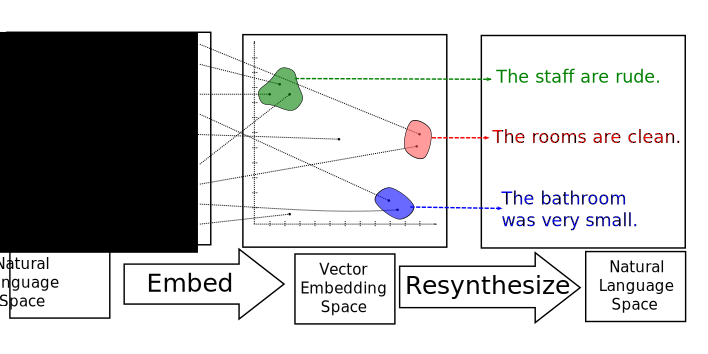
\includegraphics{./workflow}}
\end{frame}

%Room for a few more slides on Application Here

\begin{frame} {How to get Vector Repressentations?} 
	Extract form Neural Network Hidden Layer.
\end{frame}


\section{Methods}
\begin{frame} {2 minute Into To NN}
	\begin{columns} 
	\begin{column}{0.5\textwidth}
		\center\makeatletter
\tikz@def@grow@tokens{3}{1}{-1}{0}
\tikz@def@grow@tokens{3}{2}{0}{0}
\tikz@def@grow@tokens{3}{3}{1}{0}


\tikz@def@grow@tokens{5}{1}{-1}{0}
\tikz@def@grow@tokens{5}{2}{0}{0}
\tikz@def@grow@tokens{5}{3}{1}{0}
\tikz@def@grow@tokens{5}{4}{2}{0}
\tikz@def@grow@tokens{5}{5}{-2}{0}


\tikz@def@grow@tokens{7}{1}{-1}{0}
\tikz@def@grow@tokens{7}{2}{0}{0}
\tikz@def@grow@tokens{7}{3}{1}{0}
\tikz@def@grow@tokens{7}{4}{2}{0}
\tikz@def@grow@tokens{7}{5}{3}{0}
\tikz@def@grow@tokens{7}{6}{-2}{0}
\tikz@def@grow@tokens{7}{7}{-3}{0}
\makeatother

\begin{tikzpicture}[rotate=180,
sibling sep=20mm,level sep=10mm]
\def\x{\tilde{x}}
\def\a{\tilde{a}}
\def\y{\tilde{y}}
\def\b{\tilde{b}}
\def\tanh{\mathrm{tanh}}

\graph[layered layout, 
	edges={nodes={draw=none,minimum width=0mm, minimum height=0mm,
						 font=\scriptsize, inner sep=1pt}}
]{

	Input/""[draw, minimum width=1.6cm, rectangle,label=left:$\x$,label=right:Input, colored tokens={
lightgray,lightgray, black, lightgray,lightgray
}];

	hl/""[draw, minimum width=2.3cm, rectangle,
label=left:$\a$, label=right:Hidden, colored tokens={
lightgray,lightgray,gray, black, darkgray,gray,lightgray
}];
 	Output/""[draw, minimum width=1cm, rectangle,label=left:$\y$,label=right:Output, colored tokens={
lightgray, black, lightgray
}];

	Input->[edge label={$\sigma_1 \small(W_1\x+\b_1\small)$}] hl;
	hl ->[edge label={$\sigma_2 \small(W_2\a+\b_2\small)$}] Output;

};

\end{tikzpicture}
	\end{column}
	\begin{column}{0.5\textwidth}
	
			$f:\x\mapsto\y$
			$$NN\big(W_1,\b_1,..;\x\big)\approx f \big(\x\big)$$

		\colorbox{lime}{Tune:	$W_i,\b_i$}

	\end{column}
	\end{columns}
	\note[item]{But how to we get the vector representation $\x$ for the input in question?}
	\note[item]{Lets just assume we already knew it}
\end{frame}

\begin{frame} {NN with Look Up}
	\center\makeatletter
\tikz@def@grow@tokens{3}{1}{-1}{0}
\tikz@def@grow@tokens{3}{2}{0}{0}
\tikz@def@grow@tokens{3}{3}{1}{0}


\tikz@def@grow@tokens{5}{1}{-1}{0}
\tikz@def@grow@tokens{5}{2}{0}{0}
\tikz@def@grow@tokens{5}{3}{1}{0}
\tikz@def@grow@tokens{5}{4}{2}{0}
\tikz@def@grow@tokens{5}{5}{-2}{0}


\tikz@def@grow@tokens{7}{1}{-1}{0}
\tikz@def@grow@tokens{7}{2}{0}{0}
\tikz@def@grow@tokens{7}{3}{1}{0}
\tikz@def@grow@tokens{7}{4}{2}{0}
\tikz@def@grow@tokens{7}{5}{3}{0}
\tikz@def@grow@tokens{7}{6}{-2}{0}
\tikz@def@grow@tokens{7}{7}{-3}{0}
\makeatother

\begin{tikzpicture}[rotate=180]
\def\x{\tilde{x}}
\def\a{\tilde{a}}
\def\y{\tilde{y}}
\def\b{\tilde{b}}
\def\tanh{\mathrm{tanh}}

\graph[spring layout, node distance=2.1cm,
	edges={nodes={draw=none,minimum width=0mm, minimum height=0mm,
						 font=\scriptsize, inner sep=1pt}},
	word/.style={font=\itshape}
]{



	//[layered layout, level sep=1pt, level distance=1pt]{
 	I1/""[draw, minimum width=1.6cm, rectangle,label=left:$\x_{the}$, colored tokens={
lightgray,lightgray, gray, lightgray,black
}],
 	I2/""[draw, minimum width=1.6cm, rectangle,label=left:$\x_{cat}$, colored tokens={
lightgray,lightgray, black, lightgray,lightgray
}],
 	I3/""[draw, minimum width=1.6cm, rectangle,label=left:$\x_{sat}$, colored tokens={
lightgray,gray, lightgray, black, lightgray
}],
	I1->[draw=none]I2->[draw=none]I3,
Lookup[draw,font=\scriptsize]//{I1,I2,I3}	
};



	//[layered layout]{
	Input/""[draw, minimum width=1.6cm, rectangle,label=left:$\x$,label=right:Word Vector, colored tokens={
lightgray,lightgray, black, lightgray,lightgray
}],
	hl/""[draw, minimum width=2.3cm, rectangle,
label=left:$\a$, label=right:Hidden, colored tokens={
lightgray,lightgray,gray, black, darkgray,gray,lightgray
}],
 	Output/""[draw, minimum width=1cm, rectangle,label=left:$\y$,label=right:Output, colored tokens={
lightgray, black, lightgray
}],
	Input->[edge label={$\sigma_1 \small(W_1\x+\b_1\small)$}] hl,
	hl ->[edge label={$\sigma_2 \small(W_2\a+\b_2\small)$}] Output
};

word/{``Cat"}[word, label=below:word input];
word->I2;
word->[draw=none,orient=275]Input;
I2->Input;




};

\end{tikzpicture}
	\colorbox{lime}{Tune:	$W_i,\b_i,\x_j$}

\end{frame}


\begin{frame} {Sliding Window: CBOW} 
	
\end{frame}

\begin{frame} {PV DM} 
	
\end{frame}

\begin{frame} {RNN} 
	
\end{frame}

\begin{frame} {RvNN} 
	
\end{frame}

\begin{frame} {URAE} 
	
\end{frame}

\begin{frame} {Semisupervised URAE} 
	Why not do both?
\end{frame}

\section{Limitations}
\begin{frame}{Not reversible}
	Even The URAE which looks reversible, requires you to know the way out to get there.
	For RvNN decended models, we end up with a tree search problem
\end{frame}

\begin{frame}{Not semantic, enough}
	
	S/MOWE
	BRAE
\end{frame}


\section{Conclusion}
\begin{frame}{Conclusion: There}
	\begin{itemize}
		\item Too much information for people to handle
		\item but written only for people
		\item need to make machines handle Natural Language
		\item machine are good at numbers
		\item so we turn sentences into numbers.
	\end{itemize}
\end{frame}

\begin{frame}{Conclusion: and Back Again}
	\begin{itemize}
		\item Once they are vectors, operate on them
		\item Go back to sentences
		\item to go back to sentences, position needs to corespond to meaning
		\item and must have method to get back
	\end{itemize}
\end{frame}


	


\end{document}
